
\chapter{Transverse Asymmetry} \label{transv}

\paragraph{}
This chapter introduces the theory behind the transverse asymmetry. The \transv arises from interference between two scattering amplitudes, the exchange of one and two virtual photons, and is deeply connected with the Time-reversal operator. These two scattering amplitudes, given by electromagnetic interaction between the incident electron and the nucleus, are discussed in this chapter, together with the limits of the theory developed to describe the experimental data. The chapter also presents the problem of the anomalous observation of zero $A_{n}$ for lead target, made by PREX. In the end we discuss the general formula of $A_{n}$ and we study how the accuracy of a measurement varies increasing the statistics. 

\section{Description of the Process}

The Beam Normal Single Spin Asymmetry (BNSSA), which we will refer to as Transverse Asymmetry, originates from the interference of two scattering processes. The theory of the electron scattering against a spin $0$ target is extensively treated in \cite{Gorchtein_2008}.
To understand why the interference of this two scattering amplitude give rise to an asymmetry, we first have to look at the kinematics of the experiment, shown in figure \ref{fig:ScatteringSchemeFinal}

\begin{figure}[hbtp] 
\centering
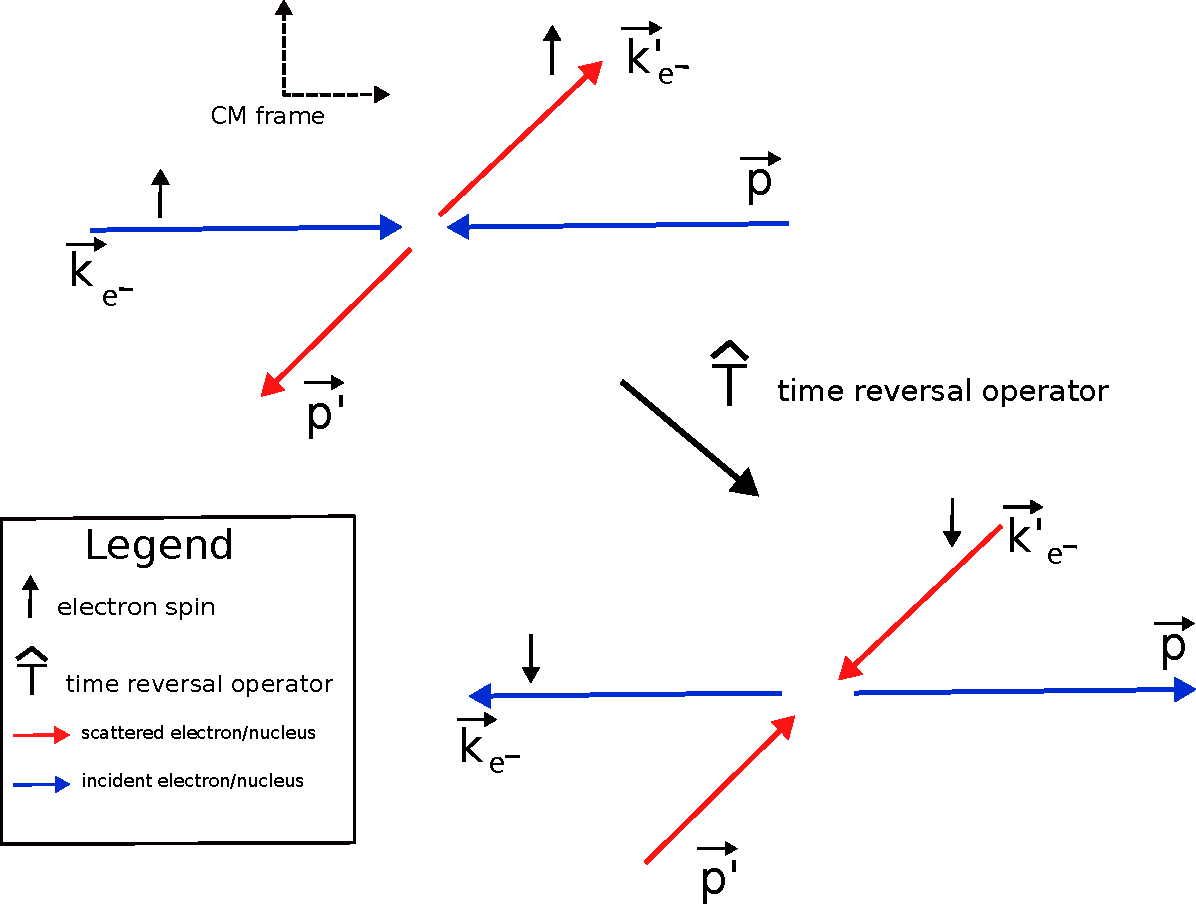
\includegraphics[width = 0.6\textwidth]{Transverse/scattering.pdf}
\caption{Scheme of the scattering process in the center of mass frame. In blue the incident electron and nucleus, in red the outgoing electron and nucleus. All the quantities are referred to the center of mass frame. The small arrow over the vector represent the electron spin, lying in the normal plane.}
\label{fig:ScatteringSchemeFinal}
\end{figure}

In the figure we can compare the two situation before and after applying the Time-reversal operator, $\hat{T}$. Looking at the picture we can understand that: 

\begin{itemize}
\item Before applying $\hat{T}$, we have the incoming electron with $\vec{k}$ momenta and the nucleus with $\vec{P}$ momenta. Applying $\hat{T}$ will exchange the incoming electron and nucleus with the outgoing electron and nucleus.
\item The $\hat{T}$ operator flips also the spin of the incoming electron.
\item Considering that the process is elastic, the kinematic is the same with and without applying the the Time-reversal operator. 
\end{itemize}

The time-reversal operator exchanges the two different cases of electron scattering with UP and DOWN polarized electron. Our goal is to measure the asymmetry between the two cross section:

\begin{equation}
A = \frac{\sigma_{\uparrow} - \sigma_{\downarrow}}{\sigma_{\uparrow} + \sigma_{\downarrow}}
\end{equation}

A non-zero asymmetry depends on how the time-reversal act on the elastic amplitude of the process. Therefore is important to see more in detail the structure of the $\hat{T}$ operator. We know that $\hat{T}$ is an anti-unitary operator that can be always decomposed as:

\begin{align*}
\hat{T} = U \cdot K
\end{align*} 
Where $U$ is an unitary operator, while $K$ is the complex conjugation operator that generates the complex conjugate of the coefficients in front of the state vectors. If we consider a ket describing a system, we have that:

\begin{equation}
Kc \ket{\alpha} = c^{*} K \ket{\alpha}
\end{equation}

Now, let's consider the total amplitude of our system. We want to apply the $\hat{T}$ operator. We assume that the amplitude of the system consist of two term, one real and one imaginary, which correspond to the two different scattering processes. Since the electromagnetic interaction conserve $CP$ symmetry, also $T$ is conserved. However the time reversal operator changes the relative sign between the real and complex terms of the scattering amplitude. Therefore, the value of the cross-section is changed when the time reversal operator is applied to the system, and this give rise to the asymmetry $A_{n}$.

\commento{\begin{equation}
H = H_{R} + i H_{Im} \quad ; \quad \hat{\Theta} H \hat{\Theta}^{-1}= \hat{\Theta}H_{R} \hat{\Theta}^{-1} + \hat{\Theta} i H_{Im} \hat{\Theta}^{-1} \Rightarrow H_{R} - i H_{Im} \neq H
\end{equation}}

At the $\alpha$ leading order, the two scattering processes that give rise to the asymmetry involve the one-photon-exchange (OPE) and two-photon-exchange (TPE) Feynmann diagrams, that are show in figure \ref{fig:FeynmannDiagrams}  

\begin{figure}[hbtp]
\[
\feynmandiagram [scale = 1, transform shape][baseline = (h), horizontal = d to j]{
	a [particle = \(e^{-}\)] -- [fermion, thick] c -- [fermion, thick ] f -- [fermion, thick] g [particle = \(e^{-}\)],
	c -- [photon, edge label = \(\gamma\)] d [blob],
	f -- [photon, edge label = \(\gamma\)] j [blob],
	h [particle = \(^{12}C\)]-- d -- [fermion, thick] j -- k [particle = \(^{12}C\)] ,
	};
\qquad \qquad \qquad
\feynmandiagram [scale = 1, transform shape][ vertical = c to d]{
	a [particle = \(e^{-}\)] -- [fermion, thick] c -- [fermion, thick] g [particle = \(e^{-}\)],
	c -- [photon, edge label' = \(\gamma\), momentum = {[arrow style = red]\(k\)}] d [blob],
	h [particle = \(^{12}C\)] -- [fermion, thick] d -- [fermion, thick] j [particle = \(^{12}C\)],
	};
\]
\caption{TPE and OPE diagrams in electron nucleus scattering.}
\label{fig:FeynmannDiagrams}
\end{figure}

The important quantity to compute the cross section is the scattering amplitude. The scattering amplitude is given by the two contributions: the exchange of a single virtual photon $A_{1}$ and the terms given by the two photon exchange $A_{2}$. In general we can write that the total scattering amplitude $S$:

\begin{equation}
S = i \dfrac{e^{2}}{Q^{2}} \overline{u}(k') [ \, m_{e} A_{2} + A_{1} \slashed{P} \,] u(k)
\end{equation}

Where in this expression, $\vec{P}$ is given by the formula

\begin{equation}
\vec{P} = \frac{\vec{p} + \vec{p}'}{2} .
\end{equation}

The $A_{1}$ term in the scattering amplitude is given by the form factor of the nucleus:

\begin{align*}
A_{1} = 2Z F_{N}(Q^{2})
\end{align*} 

Where $Q^{2}$ is the transferred momentum in the scattering process. The one photon exchange amplitude, corresponding to the right diagram in figure \ref{fig:FeynmannDiagrams}, is computed applying the feynmann rules. The first interaction vertex connect the incoming and outgoing electron. The electron is represented by a spinor, and the expression is given by: 

\begin{equation}
\overline{u}(k') (-ie \gamma^{\nu}) u(k) ,
\end{equation} 

For the other vertex, which involves the carbon nucleus, we have to apply the feynmann rules for spin 0 particles, that correspond to:

\begin{equation}
-ie(p + p')_{\mu} \cdot Z F_{N}(Q^{2}).
\end{equation}

Since the carbon is not a point like particle, the formula contains the charge form factor $Z F_{N}(Q^{2})$, while $p$ and $p'$ are the incoming/outgoing momenta of the $^{12}C$ nucleus. 
\commento{
The lagrangian term for a vertex of this type is given by the formula: 
\begin{equation}
\Lagr_{interaction} = +ieA_{\mu}(\Phi \partial^{\mu} \Phi^{\dag} - \Phi^{\dag}\partial_{\mu} \Phi)
\end{equation}}

The last term to consider is the feynmann propagator for the virtual photon:

\begin{equation}
\frac{-i \eta_{\mu \nu}}{Q^{2}}
\end{equation}

considering all this terms together gives the scattering amplitude of the one photon exchange. This first part of the scattering amplitude is T-even, and it is purely real, so it is the imaginary part of the two photon exchange amplitude which gives rise $A_{n}$. In the end, the expression that connects the scattering amplitudes to the \transv is given by:

\begin{equation} \label{eq:integral}
A_{n} = -\frac{m_{e}}{\sqrt{s}} tan \bigl (\frac{\theta_{CM}}{2} \bigl) \dfrac{\Im(A_{2})}{ZF_{N}(Q^{2})}
\end{equation}

Looking at this formula, the theoretical effort to compute the transverse asymmetry is given by the imaginary part of $A_{2}$. The calculation of this quantity is theoretically challenging, due to the fact that at energies of $\simeq \SI{1}{\giga \electronvolt}$ of incident electrons, contributions from intermediate excited states become important. Because of this, the contribution of $A_{2}$ are given by the sum of elastic intermediate state and inelastic terms, which involve hadronic excitations.

\subsection{Hadronic Tensor}

The imaginary part $A_{2}$ is related to the two-photon exchange. To compute this quantity, we have to perform an integration over the internal momenta of the electron $k_{1}$ (see figure \ref{fig:FeynmannDiagrams}). This contribution, following \cite{Gorchtein_2008}, is given by:

\begin{equation}
\Im(A_{2}) = e^{4} \frac{1}{(2\pi)^{2}} \int \dfrac{l_{\mu \nu} \cdot W^{\mu \nu}}{2E_{1} Q_{1}^{2} Q_{2}^{2}} d^{3}\vec{k_{1}}
\end{equation}

Two new terms appear in this expression. The first term is $l_{\mu \nu}$, named leptonic tensor. This term is given computing the Amplitude for the upper part of the diagram, which involve the incident and scattered electron:

\begin{equation}
l_{\mu \nu} = \overline{u}(k') \gamma_{\nu} (\slashed{k}_{1} + m_{e}) \gamma_{\mu} u(k)
\end{equation}

In this expression is immediate to recognize the feynmann rules for fermion vertex. The term $(\slashed{k_{1} + m_{e}})$ comes from the fermion propagator of the internal electron, which is:

\begin{align*}
\dfrac{i(\slashed{p} + m)}{p^{2} + m^{2}}
\end{align*}

The other term is $W^{\mu \nu}$, the hadronic tensor. For the elastic contribution this term is simply given by the feynmann rules for vertex with spin 0 particles, with the proper correction of the form factor, so we can write:

\begin{equation}
W_{\mu \nu} = \pi \delta((p + k - k_{1})^{2} - M^{2}) (2p + q_{1})_{\mu} (2p' + q_{2})_{\nu} \times Z^{2} F_{N}(Q_{1})  F_{N}(Q_{2})
\end{equation}

At this point, one can substitute in the integral above, and compute the contribution of the transverse asymmetry due to the elastic term. This first terms scales with the nuclear charge $Z\alpha$, and this is important for electron scattering with heavy nuclei. However, this mechanism is important in the energy range of few MeV, and has a minor impact, although not negligible, for higher energy, such as the energy of interest for this thesis.
For the inelastic contributions, the structure of the hadronic tensor is different. Realistic estimate are given only for nearly forward scattering angles. The hadronic tensor is given in terms of the structure functions $W_{1,2}$

\begin{equation}
W^{\mu \nu} = 2 \pi W_{1}(\omega^{2},Q_{1}^{2}) \Bigl( -g^{\mu \nu} + \dfrac{P^{\mu}q_{1}^{\nu} +  P^{\nu}q_{2}^{\mu}}{(P \overline{K})} - \dfrac{q_{1} q_{2}}{(P \overline{K})^{2}}P^{\mu}P^{\nu} \Bigl)
\end{equation}

Several assumption are made to treat this new term. The structure function, for forward scattering angles, can be approximated by a function containing the Compton form factor of the nucleus, neglecting some dependence on $Q_{1,2}$ that let to simplify the integral in equation \ref{eq:integral}. It is beyond our scope to go into a detailed description, which can be found in the articles (\cite{Gorchtein_2006}, \cite{Gorchtein_2008}, \cite{Koshchii_2021}). We emphasize however that for the estimation of the inelastic intermediate state, theoretical calculation are affected by the approximation of forward angles and other assumptions due to lack of data in the dependence of some important variables, such as the Compton form factor for carbon 12, the Compton slope parameter and the use of the approximated Callavan-Gross relation. In summary, the theoretical prediction for the \transv are reliable for small scattering angle, that correspond to lower values ​​in transfer momentum $Q$; the experimental data measure by PREX \cite{HAPPEX:2012fud} for $^{1}H$, $^{4}He$, and $^{12}C$ at $Q$ values of $\SI{0.31}{\giga \electronvolt}$, $\SI{0.28}{\giga \electronvolt}$ and $\SI{0.1}{\giga \electronvolt}$, respectively, are in agreement with the theoretical prediction. The measurement performed at MAMI for $^{12}C$ \cite{Esser:2018vdp} is with higher values of transfer momentum ($Q = \SI{0.2}{\giga \electronvolt}$) and shows a reasonable agreement with the theoretical prediction, considering also the systematic uncertainties associated to the poorly known Compton slope parameter. The model which describes the transverse asymmetry is:

\begin{equation}
A_{N} = C_{0} \cdot log(\dfrac{Q^{2}}{m_{e}^{2} c^{2}}) \dfrac{F_{Compton}(Q^{2})}{F_{ch}(Q^{2})}
\end{equation}

Where $F_{ch}$ is the charge form factor, $F_{Compton}$ is the Compton form factor of the nucleus, and $C_{0} = \dfrac{- m_{e} E_{Lab} \sigma_{\gamma p} M A}{8 \pi^{2} \sqrt(2) Z}$, where $\sigma_{\gamma p}$ is the proton photo-absorption cross section, $A$ the mass number. 
The theory presented so far is quite successful in describing the data, but it fails completely with $^{208}Pb$ nucleus, as PREX reported a measurement of $0$ transverse asymmetry \cite{HAPPEX:2012fud}. This could suggest that theory fails to describe $A_{n}$ for heavy elements; on the other hand it represents an unexpected improvement for the PV scattering experiment. It is important therefore to repeat independently the measurement of the $A_{n}$ for $^{208}Pb$, to confirm or question the result reported by PREX.

\begin{figure}[hbtp]
\centering
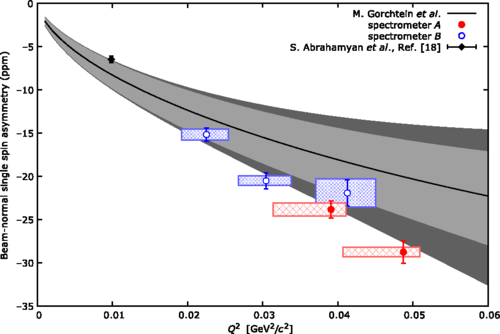
\includegraphics[scale = 0.5]{Transverse/medium.png}
\caption{Transverse asymmetry measured at MAMI for $^{12}C$ target \cite{Esser:2018vdp}. Theoretical calculation for $E_{beam} = \SI{570}{\mega \electronvolt}$  is shown.}
\end{figure}

\section{Concept of the Experiment}

We have seen so far how the Transverse Asymmetry is related to the interference between two scattering amplitude, and the theoretical model used to describe the process. The goal from an experimental point of view is to measure this quantity. The challenge is to obtain a valid measure of $A_{n}$, which is of the order of $20$ part per million (ppm), taking into consideration all the possible effects that can interfere. To measure $A_{n}$, the straightforward method is to prepare an electron beam, with polarized electron, and send it to a fixed target. The scattered electrons are then collected by a detector placed at a certain angle, with the transverse asymmetry obtained by:

\begin{equation}
A_{N} (Q) = \dfrac{N_{\uparrow}(Q) - N_{\downarrow}(Q)}{N_{\uparrow}(Q) + N_{\downarrow}(Q)}  
\end{equation} 

In an experiment of this type, several requirements need to be satisfied, in order to measure $A_{n}$ effectively:

\begin{itemize}
\item The accelerator must produce a polarized beam, stable over the time, with an high polarization percentage, in order to amplify the effect.
\item The Beam energy needs to be quite stable, and should not depend on the Polarization state of the electrons. A change in the Beam energy associated with the polarization state can lead to a different count rate for $N_{\uparrow}$ and $N_{\downarrow}$, and would create an undesired contribution that adds to the $A_{n}$.
\item The beam must be correctly aligned with the target, with a stable position. If the position of the target changes according to the polarization of the electrons, it will produce another contribution to the total asymmetry.
\item The beam current should not depend on the polarization state of the electrons. If the beam source depends on the polarization, we will have a difference in the event rate and then another false asymmetry.
\item It is necessary to reject possible double elastic scattering events, which may contribute to the total asymmetry. 
\end{itemize}

All this demands can be satisfied with an accelerator that has stabilization devices with great precision and that can sustain high beam intensities. This last request is necessary to accumulate enough statistics to measure the transverse asymmetry with an accuracy about 1 ppm, in view of the future PV experiments. We can quantify how the statistical error varies according to the amount of data available. With the assumption that $N_{\uparrow,\downarrow}$ are gaussian distributed variables, we can compute the expected variance

\begin{equation}
Var[A_{n}] = \dfrac{1 - A^{2}}{N_{\uparrow} + N_{\downarrow}} 
\end{equation}

For a single measurement of the $A_{n}$. For multiple $n$ measurements, the variance scales as $\frac{1}{n}$.
Because $A_{n}$ is expected to be smaller respect to 1, we can approximate the above formula:
\begin{equation} 
V[A_{n}] = \dfrac{1}{2N \cdot n}  \label{eq:Error}
\end{equation}

The error associated to the reconstructed asymmetry is the square root of the above quantity. If we impose that the error must be $\le 1ppm$ we can easily obtain that the quantity $n\cdot N$:

\begin{align*}
n\cdot N > \frac{1}{2} \cdot 10^{12}
\end{align*} 

We will see later that achievable rates $N_{\uparrow,\downarrow}$ are in the range (20000,60000) counts per event for a carbon target. This number can not be increased at will by acting on the beam current. The first reason is oblivious: the beam source can produce only a certain amount of electrons before loosing, furthermore a beam with great intensity for an extended periods of time can damage the carbon target up to the risk of melting it. Another idea might be to increase the thickness of the target, to take advantage of the larger cross section. However, by doing so, the number of double scattering events would be increased. To avoid the problem of the double scattering, the nuclear physic community which deals with PV experiments respects the convention that the target thickness should be less than the $10 \%$ of the radiation length of the material.
